\documentclass[a4paper, 11pt, oneside]{report} 
\usepackage[utf8]{inputenc}
\usepackage[dutch]{babel}
\usepackage{diagbox}
\usepackage{amsmath}
\usepackage{amsfonts}
\usepackage{amssymb}
\usepackage{graphicx}
\usepackage{caption}
\usepackage[table,xcdraw]{xcolor}
\usepackage[toc,page]{appendix}
\usepackage{hyperref}
\usepackage{titlesec}
\usepackage{listings}
\usepackage{float}
\usepackage{tikz}
\usetikzlibrary{trees}
\usepackage{tikz-qtree}
\usepackage{graphicx}
\usepackage{fancyref}
\usepackage{wrapfig}
\usepackage{url}
\usepackage{pdflscape}
\usepackage{fancyvrb}
\usepackage{fancyhdr}
\graphicspath{ {Afbeeldingen/} }
\usepackage{subfig}
\usepackage{tabularx}
\usepackage{apacite}
\usepackage{longtable}
\usepackage{titlecaps}
%\usepackage[T1]{fontenc}
\usepackage{titlesec, blindtext, color}
\definecolor{gray75}{gray}{0.75}
\newcommand{\hsp}{\hspace{20pt}}
\usepackage{pdfpages}
\usepackage{booktabs}
\usepackage{listings}

\newcolumntype{L}[1]{>{\raggedright\arraybackslash}p{#1}}

\titleformat{\chapter}[hang]{\huge\bfseries}{\thechapter\hsp\textcolor{gray75}{|}\hsp}{0pt}{\Large\bfseries}

\makeatletter
\newcommand\tagreq[2]{#1\def\@currentlabel{#1}\label{#2}}
\makeatother

\def\checkmark{\tikz\fill[scale=0.4](0,.35) -- (.25,0) -- (1,.7) -- (.25,.15) -- cycle;} 
\def\figureautorefname{Figuur}
\def\sectionautorefname{Paragraaf}
\def\chapterautorefname{Hoofdstuk}
\def\tableautorefname{Tabel}
\DeclareRobustCommand{\VAN}[3]{#2} % set up for citation

%% Sets page size and margins 
\usepackage[a4paper,top=3cm,bottom=3cm,left=3cm,right=3cm,marginparwidth=1.75cm]{geometry}

\definecolor{dkgreen}{rgb}{0,0.6,0}
\definecolor{gray}{rgb}{0.5,0.5,0.5}
\definecolor{mauve}{rgb}{0.58,0,0.82}

\lstset{frame=tb,
	language=Java,
	aboveskip=3mm,
	belowskip=3mm,
	showstringspaces=false,
	columns=flexible,
	basicstyle={\small\ttfamily},
	numbers=none,
	numberstyle=\tiny\color{gray},
	keywordstyle=\color{blue},
	commentstyle=\color{dkgreen},
	stringstyle=\color{mauve},
	breaklines=true,
	breakatwhitespace=true,
	tabsize=3
}

\author{M.W.J. Berentsen}
\font\myfont=cmr12 at 40pt
\title{\myfont Drone mesh netwerk simulatie}
\usepackage{titling}

\newcommand{\subtitle}[8]{%
	\posttitle{%
		\par\end{center}
	\begin{center}\large#1\end{center}
	\vskip0.5em
	\begin{center}\large#2\end{center}
	\begin{center}\large#3\end{center}
	\begin{center}\large#4\end{center}
    \begin{center}\large#5\end{center}
    \begin{center}\large#6\end{center}
    \begin{center}\large#7\end{center}
    \begin{center}\large#8\end{center}
	\vskip0.5em}%
}

\subtitle{Onderzoeksrapport}{HAN Arnhem}{561399}{MWJ.Berentsen@student.han.nl}{Versie 1}{Alten Nederland B.V.}{Docent: J. Visch, MSc}{Assessor: ir. C.G.R. van Uffelen}

\setlength{\parindent}{0pt}
\setlength{\parskip}{5pt plus 2pt minus 1pt}



\hypersetup{colorlinks=true, urlcolor=red,citecolor=black,linkcolor=blue}  % Colours hyperlinks in blue, but this can be distracting if there are many links.
\setcounter{tocdepth}{2}



\begin{document}
\begin{figure}
\begin{center}
\includegraphics[scale=0.1]{alten}\end{center}
\end{figure}
\maketitle

%\section*{Voorwoord}
%\addcontentsline{toc}{section}{\protect\numberline{}Voorwoord}
%\pagebreak

\tableofcontents
\clearpage
%\section*{Begrippenlijst}

% Please add the following required packages to your document preamble:
% \usepackage[table,xcdraw]{xcolor}
% If you use beamer only pass "xcolor=table" option, i.e. \documentclass[xcolor=table]{beamer}
%\begin{table}[H]
%\centering

%\label{begrippen}
%\begin{tabular}{|l|l|}
%\hline
%\rowcolor[HTML]{C0C0C0}
%Term        & Omschrijving                                                         \\ \hline
%term        & Omschrijving                                                      	\\ \hline

%\end{tabular}
%\caption{Begrippenlijst}
%\end{table}

%\clearpage

%\section*{Samenvatting}
%\addcontentsline{toc}{section}{\protect\numberline{}Samenvatting}
%\pagebreak

\chapter*{Samenvatting}

Optioneel een samenvatting van het onderzoek. Hier kunnen anderen snel inzicht krijgen in wat jij hebt onderzocht en wat je conclusie is.
\begin{itemize}
	\item Kunnen derden snel inzicht krijgen in jouw onderzoek?
	\item Staat de conclusie erin vermeld?
\end{itemize}
\hrule

\chapter{Inleiding}
\label{chapter:inleiding}


De inleiding beschrijft:
\begin{itemize}
\item Waarvoor het onderzoek gedaan wordt;
\item Beschrijf waarom het onderzoek nu wordt uitgevoerd;
\item Het doel van het onderzoek.
\end{itemize}
\hrule

Het volgende onderzoek rapport wordt uitgevoerd ten behoeve van de het afstudeerproject van Maurice Berentsen, Hogeschool van Arnhem en Nijmegen.


\chapter{Hoofd- en deelvragen}
In dit hoofdstuk worden de hoofd- en deelvragen genoemd en onderbouwd.
Er wordt een scope bepaalt met wat er onderzocht wordt en dus ook wat niet.
Vervolgens wordt de onderzoeksmethode toegelicht en beargumenteerd.
Tenslotte wordt de invloed van het onderzoek op het afstudeerproject beschreven.

\section{Hoofdvraag}
Het doel van dit onderzoeksrapport is het beantwoorden van de volgende opgesteld hoofdvraag:
\begin{quotation}
\textit{Hoe kan een netwerkmodule een groep van ongeveer 100 drones voorzien van een onderling meshnetwerk die snel reageert op uitval van netwerkpunten?}	
\end{quotation}
Doordat de uitvoerende student van dit onderzoek niet beschikt over een certificaat om met drones te mogen vliegen behoudt dit onderzoek zich tot een simulatie.
Van de netwerkmodule wordt wel een fysiek prototype ontwikkeld.

\section{Deelvragen}

Om de hoofdvraag te kunnen beantwoorden zijn er de volgende deelvragen opgesteld:

\begin{itemize}
	\item Welke simulatie software is geschikt om een netwerk van ongeveer 100 drones in na te bootsen?
	\item Wat is de grote van de payload die een netwerkmodule aangesloten op een drone moet versturen om nuttig te zijn voor een aansturingssysteem?
	\item Welke mesh netwerk hardware is geschikt voor het onderling verbinden van drones?
	\item Welke mesh netwerk libary is geschikt voor de te gebruiken hardware?
	\item Hoe gedraagt een node uit het mesh netwerk zich bij slecht of geen bereik?
	\item Wat kan er toegevoegd worden aan de communicatie van de netwerkmodule om snel [TODO snel definiëren] achter uitval te komen?
	\item Wat is minimaal benodigd in een simulatie om abstracte drone te representeren?
\end{itemize}

\section{Onderzoeksmethode}
De onderzoeksmethodes volgen de structuur van de \textit{ICA methodenkaart} \cite{MethodenKaart}.
De methodenkaart is een onderzoek framework voor professionals in ICT en media.
Het ontwerp van het framework gaat uit van het idee van triangulatie.
Triangulatie is het combineren van verschillende theorieën, methoden of databronnen om zo tot betere antwoorden te komen op je onderzoeksvragen \cite{ICAoates}. 
Door het definiëren van zo geheten werkplaatsen en hun samenhang geeft het de onderzoeker een set van methoden en technieken. 
De vijf verschillende werkplaatsen binnen het framework zijn: \textit{lab, veld, showroom, bieb en werkplaats}.

\begin{figure}[H]
	\begin{center}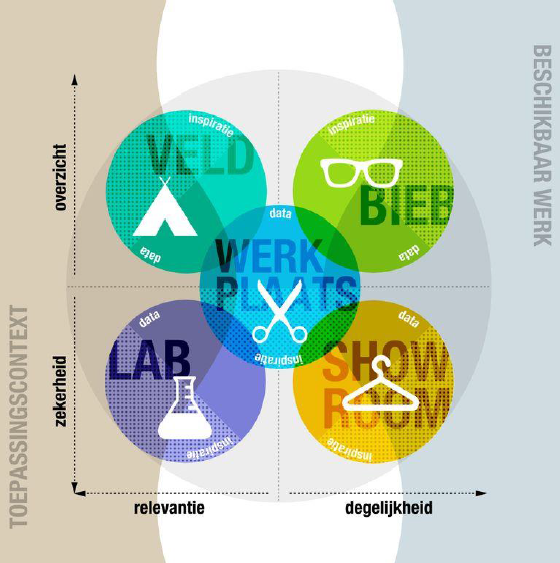
\includegraphics[width=0.5\linewidth]{Methodenkaart}\end{center}
	\caption{De vijf werkplaatsen binnen het framework en hun systematiek. Overgenomen uit \textit{De informatieprofessional 3.0}  van \protect\citeA{MethodenKaart}  }
	\label{fig:methodenkaart}
\end{figure}

\subsection{De gekozen onderzoeksmethodes}

De deelvragen gaan gedeeltelijk over keuzes van gebruik. 
Welke software en hardware is geschikt, is een vraag die veel naar voren komt.
Hieruit valt te concluderen dat de onderzoeker zich nog aan het oriënteren is.
"De onderzoeksruimte bieb bevat een verzameling methoden en technieken die dienen tot oriëntatie op beschikbaar werk."\cite{MethodenKaart}
Daarom wordt er gekozen om een bieb onderzoek uit te voren naar de deelvragen die gaan over geschiktheid.
Dit zodat de onderzoeker zich nog kan oriënteren naar het beschikbare aanbod en nog op nieuwe deelvragen kan komen. 

Lab onderzoek wordt pas later uitgevoerd omdat niet alle hardware voor handen is, maar ook omdat er niet genoeg tijd voor beschikbaar is.
\citeauthor{MethodenKaart} zegt het volgende over lab onderzoek: De onderzoeksruimte lab bevat methoden die geschikt zijn om de oplossing te toetsen aan een aspect van de toepassingscontext.
Daarom is het lab onderzoek geschikt voor het moment waarop de hardware beschikbaar is en de onderzoeker het gedrag hiervan exact in kaart wil brengen en wil bewijzen dat de gestelde eisen behaald worden.

\citeA{ICAoates} stelt dat een systeem bouwen 'bewijs' is dat een nieuw soort toepassing gebouwd kan worden. Als dit het doel is heeft het onderzoek waarschijnlijk hoofdzakelijk een werkplaats karakter, maar alle andere onderzoeksruimtes kunnen een rol spelen.
Gedurende het huidige onderzoek zal er door de onderzoeker software geschreven worden om bewijs te leveren dat een netwerkmodule een groep drones kan voorzien van een onderling netwerk.
Daarom past de werkplaats onderzoeksruimte goed bij dit onderzoek.


\section{Invloed op het project}



\chapter{Criteria}
\label{chapter:criteria}
Maak hier een lijst met criteria aan de hand van de hoofd- en deelvragen.
\begin{itemize}	
\item Zijn de criteria duidelijk opgesteld?
\item Waar moet de oplossing aan voldoen, staat dit erin?
\end{itemize}
\hrule

In \autoref{tab:criteria} worden codes gebruikt als naam voor de criteria, wat deze betekenen wordt eerst toegelicht:
\begin{itemize}
	\item ALG: Een algemene eis die in elke onderzoek meegenomen moet worden.
	\item SK: Een eis die gesteld worden in de keuze naar simulatie software.
	\item DR: Een eis voor de te gebruiken drone in de simulatie.
	\item PH: Eisen opgesteld aan het hardware prototype.
\end{itemize}

\begin{longtable}{|l|l|l|}
	\hline
	\rowcolor[HTML]{C0C0C0} 
	Naam & Beschrijving \\ \hline
	%\endfirsthead
	%
	\endhead
		\hypertarget{alg1}{ALG1}	&Is voorzien van API documentatie.        \\ \hline
		\hypertarget{alg2}{ALG2}	&Ondersteunt aansturing vanuit C++ .    \\ \hline
		\hypertarget{alg3}{ALG3}	&\begin{tabular}[c]{@{}l@{}}Heeft ondersteuning voor het Linux platform Ubuntu 18.04\end{tabular}        \\ \hline
		\hypertarget{alg4}{ALG4}	&Software is gratis in gebruik voor studenten        \\ \hline
		\hypertarget{sk1}{SK1}		&\begin{tabular}[c]{@{}l@{}}Heeft ondersteuning voor UAV (unmanned air vehicle) ook wel drone genoemd\end{tabular} \\ \hline
		\hypertarget{sk2}{SK2}		&\begin{tabular}[c]{@{}l@{}}Ondersteunt de simulatie van locatie bepaling sensoren zoals GPS.\end{tabular}        \\ \hline
		\hypertarget{sk3}{SK3}		&\begin{tabular}[c]{@{}l@{}}Heeft een kant en klare oplossing voor simulatie van externe krachten zoals wind.\end{tabular}        \\ \hline
		\hypertarget{sk4}{SK4}		& Heeft een ingebouwde pathfinding oplossing.        \\ \hline
		\hypertarget{sk5}{SK5}		& Ondersteunt ROS als middleware.        \\ \hline
		\hypertarget{sk6}{SK6}		& Ondersteunt de detectie van botsingen.        \\ \hline
		\hypertarget{sk7}{SK7}		& Ondersteunt de simulatie 100 drones tegelijk.        \\ \hline
		DR1		& De drone is een quadcopter.        \\ \hline
		DR2		& De drone is is voorzien van een API voor aansturing op basis van coördinaten.       \\ \hline
		DR3		& De API sluit aan op de middleware ROS melodic.        \\ \hline
		DR4		& De drone is bruikbaar binnen de gekozen simulatie software.        \\ \hline%TODO gekozen software toevoegen
		DR5		& De drone moet een kleine goedkope drone representeren.        \\ \hline
		\hypertarget{ph1}{PH1}		& Ondersteunt een bereik van minimaal 100 meter.  \\ \hline
		\hypertarget{ph2}{PH2}		& Ondersteunt het gebruik van grid networking om tot een mesh te kunnen komen.  \\ \hline
		\hypertarget{ph3}{PH3}		& Maakt gebruik van een openbare bandbreedte.\\ \hline
		\hypertarget{ph4}{PH4}		& De antenne mag niet meer dan 10 euro kosten. \\ \hline
		PH5		& Moet zuinig in gebruik van stroom zijn. TODO beter defineren \\ \hline
		PS1		& Ondersteund een mesh netwerk van minimaal 100 nodes. \\ \hline
		PS2		& Het netwerk is zelf herstellend. \\ \hline
		PS3		& Ondersteunt het draaien op een raspberry pi of een ardunio (UNO of NANO). \\ \hline
		PS4		& Ondersteunt het versturen van zelfgemaakte berichten. \\ \hline
		
	\caption{Opgestelde criteria}
	\label{tab:criteria}
\end{longtable}

\chapter{Literatuur}


\section{Welke simulatie software is geschikt om een drone in na te bootsen?}
\label{sec:welkesim}
Voor het onderzoek wordt gebruik gemaakt van een simulatie omgeving.
Welke software wordt gebruik staat vastgesteld in deze paragraaf.
De keuze van software wordt bepaald door het uitvoeren van de bieb onderzoeksmethode. 
In de \autoref{tab:criteria} staan de criteria toegelicht waar de simulatie software aan moet voldoen.
Als hoofdcriteria wordt een lijst opgesteld met simulatoren die ondersteuning hebben voor ROS.
Vervolgens worden deze aan de hand van een kruistabel onderworpen aan de andere criteria.
Deze techniek is gebaseerd op de "Comparison Chart" van \cite{CMDmethod} uit de "\textit{CMD Methods Pack}"

De kandidaten zijn:
\begin{itemize}
	\item \href{https://www.energid.com/actin}{Actin} is een simulatie framework van het bedrijf Energid. Het is in staat om de beweging van verschillende robots gelijktijdig aan te sturen.
	\item \href{http://gazebosim.org/}{Gazebo} is een opensource robot simulatie framework bijzonder geschikt voor het simuleren van robotica in outdoor omgevingen door de uitgebreide Physics Engine Support.
	\item \href{http://www.coppeliarobotics.com/}{V-REP (Virtual Robot Experimentation Platform)} is een platform geschikt voor het snel bouwen van robot prototypes.
	\item \href{https://cyberbotics.com/}{Webots} is een open source-ontwikkelomgeving die wordt gebruikt voor het modelleren, programmeren en simuleren van mobiele robots.
	\item \href{http://openrave.org/}{OpenRAVE} biedt een ontwikkelomgeving voor het testen van motion planning algoritmes aan de hand van simulaties.
\end{itemize}

\begin{table}[H]
	\centering
	\begin{tabular}{l|*{10}r}
		%\backslashbox{Input}{Output} & int8\_t & int16\_t & int32\_t & uint8\_t & uint16\_t & uint32\_t \\
		\diagbox[width=2.7cm, height=2.4cm]{\raisebox{5pt}{\hspace*{0.25cm}Simulator}}{\raisebox{-1.27cm}{\rotatebox{90}{Eis}}} & \raisebox{-0.25cm}{\rotatebox{90}{\hyperlink{alg1}{ALG1}}} & \raisebox{-0.25cm}{\rotatebox{90}{\hyperlink{alg2}{ALG2}}} & \raisebox{-0.25cm}{\rotatebox{90}{\hyperlink{alg3}{ALG3}}} & \raisebox{-0.25cm}{\rotatebox{90}{\hyperlink{alg4}{ALG4}}} &
		\raisebox{-0.25cm}{\rotatebox{90}{\hyperlink{sk1}{SK1}}} & \raisebox{-0.25cm}{\rotatebox{90}{\hyperlink{sk2}{SK2}}} &
		\raisebox{-0.25cm}{\rotatebox{90}{\hyperlink{sk3}{SK3}}} & \raisebox{-0.25cm}{\rotatebox{90}{\hyperlink{sk4}{SK4}}} &
		\raisebox{-0.25cm}{\rotatebox{90}{\hyperlink{sk5}{SK5}}} & \raisebox{-0.25cm}{\rotatebox{90}{\hyperlink{sk6}{SK6}}} \\
		\midrule\\
		\hspace*{0.25cm}Actin 	& \checkmark & \checkmark 	& \checkmark & x 		  & \checkmark & x 			& \checkmark & x 		  &\checkmark & \checkmark	\\ \\
		\hspace*{0.25cm}Gazebo 	& \checkmark & \checkmark 	& \checkmark & \checkmark & \checkmark & \checkmark & \checkmark & \checkmark &\checkmark & \checkmark	\\ \\
		\hspace*{0.25cm}V-REP 	& \checkmark & x 			& \checkmark & \checkmark & \checkmark & \checkmark & \checkmark & \checkmark &\checkmark & x	\\ \\
		\hspace*{0.25cm}Webots 	& \checkmark & \checkmark 	& \checkmark & \checkmark & \checkmark & \checkmark & \checkmark & \checkmark &\checkmark & \checkmark 	\\ \\
		\hspace*{0.25cm}OpenRAVE& \checkmark & \checkmark	& \checkmark & \checkmark & x 		   & \checkmark & \checkmark & \checkmark &\checkmark & x 	\\ \\
		\bottomrule
	\end{tabular}%
	\caption{Kruistabel simulatiekeuze}
	\label{tab:kruissimkeuze}%
\end{table}%

In de \autoref{tab:kruissimkeuze} komt de simulatie software van Gazebo en Webots naar voren als enige simulatoren die voldoen aan alle gestelde eisen.
Het is nu zaak om te uit te zoeken welke van de twee het meest geschikt is voor het uitvoeren van dit onderzoek.

\subsection{Gazebo of Webots?}
In januari 2018 hebben \citeauthor{RobotCompare} een publicatie geschreven waarin zij drie simulatoren vergelijken in het aanbod van features en performance. 
Zij hebben een vergelijking gedaan tussen V-REP, Gazebo en ARGoS. 
ARGoS is niet meegenomen in de overweging omdat het geen ondersteuning heeft voor ROS.

In de conclusie van de publicatie komt Webots als het meest gebruiksvriendelijk naar voren in het gebruik en is in het bezit van de meeste features.
Het grote nadeel van Webots is dat het veel kracht vraagt van de computer waardoor het niet geschikt is voor de simulatie van veel drones tegelijk.

Daarmee komt de keuze uit op Gazebo. 
De resultaten in de publicatie van \citeA{RobotCompare} tonen aan dat de software in staat is om veel drones tegelijk aan te kunnen sturen.
\citeA{RobotCompare} geven als nadeel aan Gazebo dat de software niet in staat is om 3d meshes te manipuleren, de user interface niet innovatief is en Gazebo soms problemen met dependencies door de verschillende versies van ROS.
Dit laatste brengt een risico met zich mee voor het onderzoek daarom is het ook zaak dat dit als criteria meegenomen word in de deelvraag van \autoref{sec:dronekeuze} \nameref{sec:dronekeuze}. 

\subsection{Conclusie}
Voor het onderzoek wordt Gazebo gebruikt omdat het voldoet aan de gestelde \nameref{chapter:criteria}.
De meest recente versie van Gazebo, die niet meer beta is op 19 februari 2019, is Gazebo 9.
Deze versie vereist het gebruik van ROS Melodic volgens haar eigen website  (\href{http://gazebosim.org/tutorials?tut=ros_wrapper_versions}{zie link}).

\section{Wat is de grootte van de payload die een netwerkmodule aangesloten op een drone moet versturen om nuttig te zijn voor een aansturingssysteem?}

De payload is het gedeelte van een bericht die vrij is naar de gebruiker om invulling te geven.
De maximale grote van een payload verschilt per protocol.
Om een keuze te kunnen maken waar de hardware en het bijhorende protocol aan moet voldoen is het dus zaak om eerst te weten hoe groot deze vrije payload ruimte moet zijn.

Het doel van de berichten is om ze zo kort als mogelijk samen te stellen. 
Daarom is het belangrijk om de structuur van de berichten zo klein mogelijk te houden.
Om deze reden wordt niet gekeken naar een tekstuele serialisatie mogelijkheden zoals XML, YAML, JSON maar naar binaire mogelijkheden omdat deze veel efficienter zijn \cite{binary}.

\subsection{Binaire serialisatie voor het samenstellen van berichten} 

"Binary Serialization is converting the object in binary format and being able to store it in a storage medium"\cite{binary}. 
Het binair samenstellen van informatie is een efficiënte manier omdat de data met een minimale overhead wordt samengesteld \cite{binaryMessaging}
Het nadeel die deze wijze met zich meebrengt is dat het resultaat van het bericht niet meer makkelijk leesbaar is voor mensen.
Voor dit project ligt daar geen focus op dus is dit nadeel te verwaarlozen.

\citeA{binaryMessaging} hebben onderzoek gedaan naar een efficiënte manier naar de inzet van binaire berichten te vervanging van tekstuele serialisatie.
Hoewel dat in het huidige onderzoek niet het geval is kan er wel geleerd worden van de manier van bericht gebruik.
\citeA{binaryMessaging} tonen in hun onderzoek aan dat berichten vaak een herhalende structuur hebben en dat dit een onnodige overhead creëert in de berichten.
Een voorbeeld maken \citeA{binaryMessaging} zichtbaar in \autoref{fig:jsonxml} waarover zij het volgende zeggen: "While JSON  compared  with  XML,  eliminated  parameter  name redundancy, it keeps repeating (red box) the definition of each field  for  each  serialized  element  (green  box)". 
\begin{figure}[H]
	\begin{center}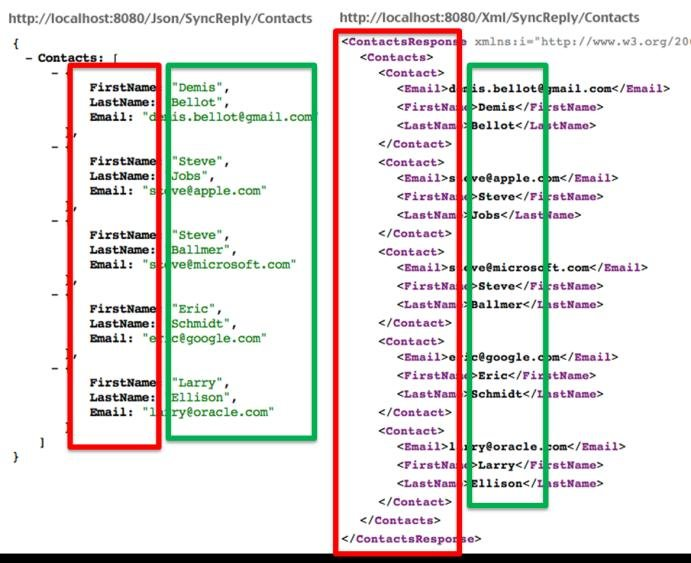
\includegraphics[width=0.5\linewidth]{JSONandXML.jpeg}\end{center}
	\caption{JSON and XML messages. Overgenomen uit \textit{International Journal of Computer Applications}  van \protect\citeA{binaryMessaging}  }
	\label{fig:jsonxml}
\end{figure}

Wat zij hebben gedaan om dit op te lossen is het apart versturen van de parameternamen zodat deze in de opvolgende berichten van dat type niet meer nodig is.
Het systeem die bedacht is geeft een enorme flexibiliteit omdat er van te voren nog geen bericht types bekend hoeven te zijn.
Deze flexibiliteit is alleen niet van toepassing op het doel van dit project, daarom kan de student in zijn software al van te voren berichttypes samenstellen waardoor er de overhead nog kleiner gemaakt wordt.
Voor nu wordt er vanuit gegaan dat 1 byte genoeg zal zijn omdat de communicatiesoftware van de netwerkmodule niet meer dan 256 ($2^{8}$) berichtentypes hoeft te ondersteunen.
Mocht het blijken dat dit toch niet genoeg is kan er er een byte toegevoegd worden waardoor er 65536 ($2^{16}$) types mogelijk zouden zijn.
Daarnaast moet een bericht om nuttig te zijn voor het netwerk altijd aan een apparaat gekoppeld kunnen worden.
De opdracht gaat over een netwerk van ongeveer 100 drones dit past ruim in een byte.


Hiermee komt het eerste deel van het bericht dus al tot stand het telt nu minimaal 2 bytes.

\begin{table}[H]
	\centering
	\begin{tabular}{|l|l|l|}
		\hline
		\rowcolor[HTML]{C0C0C0} 
		ID & Berichttype & overig \\ \hline
		00 tot FF   & 00 tot FF       & ?      \\ \hline
	\end{tabular}
	\caption{Berichtsamenstelling met type aanduiding}
	\label{tab:serialstart}
\end{table}

\subsection{Wat is de grootte van een bericht voor de locatie bepaling van drones?}

Om duidelijk te maken wat nuttig voor het systeem wordt als eerste de basis informatie vastgesteld. 
De huidige locatie is essentieel voor de verdeling van de drones.
Omdat de drones zich kunnen verplaatsen is naast de locatie ook het tijdstip waarop het bericht verstuurd wordt van belang.

\subsubsection*{Coördinaat vanuit de informatie van de GPS module}
Een positie van een locatie wordt aangeduid door coördinaten te gebruiken.
Deze worden bepaald door het gebruik van een GPS module aan boord van het systeem.
GPS modules gebruiken triangulatie van satellietsignalen om hun positie te bepalen.  

Een coördinaat is opgebouwd door de aarde te verdelen in graden over de assen latitude (horizontaal) en longitude (verticaal).
Een coördinaat loopt van -180 tot 180 graden.
De aarde heeft een omtrek van 40.07.5161,2 meter gedeeld door 360 graden levert dit per graad een stap op van 111,32 kilometer. 
Het volgende programma laat zien dat een float gebruikt kan worden in dit geval voor een accuraatheid van 5 cijfers achter het decimaal.

\begin{lstlisting}
#include <stdio.h>

float exampleFloatPositive = 179.1234567890;
float exampleFloatNegative = -179.1234567890;

int main( int argc, const char* argv[] )
{
	printf( "postive  float =  %f\n", exampleFloatPositive );
	printf( "negative float =  %f\n", exampleFloatNegative );
}
\end{lstlisting}
 
Door een coördinaat te gebruiken van 5 cijfers achter het decimaal kan een plek op aarde met een precisie van ongeveer 1,10 meter nauwkeurig aangeven worden.
Het is gebruik hiervan is realistisch omdat met alleen realtime GPS data de accuraatheid ongeveer 4 meter is \cite{GPSaccu}.
Er wordt per as een float gebruikt dit houdt in dat minimaal 8 bytes nodig zijn voor een coördinaat.
Dit is 4 bytes per float en exclusief de separator. 

\subsubsection*{Hoogte van de drone}
\citeA{GPSheight} hebben onderzoek gedaan naar de accuraatheid van de hoogtebepaling bij drones. 
Uit dit onderzoek is gebleken dat een continue vliegende drone een accuraatheid heeft van ongeveer twee meter.
Hieruit is te halen dat het geen zin heeft om op centimeter niveau de hoogte van een drone aan te geven.
Op het moment dat er een signed integer van 16 bits gebruikt zou worden kan er een afstand van 32.767 meter zowel boven als onder zeeniveau verstuurd worden.
Het is een realistische waarde om te gebruiken aangezien de grootste hoogte die gebruik kan worden dan 32 kilometer is.
Deze hoogte is al ver in de stratosfeer en al boven het niveau de weerballon halen. 
De keuze om een signed integer te gebruiken is om ondersteuning te bieden aan plekken onder het zeeniveau waarvan Nederland een groot voorbeeld is.

Voor de hoogte moeten 2 bytes gereserveerd worden. 

\subsubsection*{Tijd vanuit de GPS module}

De drone maakt al gebruik van de GPS module voor de positiebepaling.
In de berichten die de GPS module ontvangt van de satellieten wordt ook de tijd meegestuurd.
Deze tijd is volgens \cite{GPSaccu} in 95 procent van de gevallen accuraat tot 40 Nano seconden. 
In het geval van het drone netwerk is dit veilig te gebruiken als bron voor tijd.
De tijd zal aangegeven worden in het unix time format zodat deze meteen de datum met zich draagt.
Unix time maakt gebruik van 32 bits formaat, er is gekozen voor een unsigned variant aangezien er geen interesse is naar data voor 1 januari 1970 ook wel epoch genoemd.

Voor de tijd en datum worden 4 bytes gereserveerd.

\subsubsection*{Conclusie}  

De bovenstaande sub paragrafen kunnen samengesteld worden tot een bericht waarin alle informatie zit die nodig is om te bepalen waar een drone zich op een moment bevindt.
Een systeem kan met dit bericht in ieder geval elke drone afzonderlijk in kaart brengen.

\begin{table}[H]
	\centering
\begin{tabular}{l|l|l|l|l|l|l|}
	\cline{2-7}
	& \cellcolor[HTML]{C0C0C0}ID & \cellcolor[HTML]{C0C0C0}\begin{tabular}[c]{@{}l@{}}Bericht \\ type\end{tabular} & \cellcolor[HTML]{C0C0C0}latitude & \cellcolor[HTML]{C0C0C0}longitude & \cellcolor[HTML]{C0C0C0}hoogte & \cellcolor[HTML]{C0C0C0}tijd \\ \hline
	\multicolumn{1}{|l|}{\cellcolor[HTML]{C0C0C0}\begin{tabular}[c]{@{}l@{}}Aantal\\ Bytes\end{tabular}} & 1                          & 1                                                                               & 4                                & 4                                 & 2                              & 4                            \\ \hline
\end{tabular}
 \caption{Locatie bericht in bytes}
\label{tab:locatiebericht} 
\end{table}
In \ref{tab:locatiebericht} is het aantal bytes te zien benodigd voor een locatie bericht.
Het totaal aantal bytes voor dit bericht is 16 bytes.
Later moet er gekeken worden of iets aan een bericht toegevoegd kan worden om uitval sneller te detecteren. 
Desondanks het nog niet bekend is wat dit is kan er vanuit gegaan worden dat er niet meer dan 4 bytes nodig zullen zijn.

Concluderend wordt voor dit bericht een grootte van 20 bytes aangehouden waarbij 16 bytes het minimum is.
 
\subsection{Wat is de grootte van een bericht waarin een netwerkmodule zijn verbinding met anderen aangeeft}


\chapter{Oplossingsrichtingen}

\begin{itemize}
\item Beschrijf je hoe jouw oplossingsrichting de hoofdvraag beantwoord?
\item Beschrijft de oplossingsrichting de mogelijkheden?
\item Staat hier "Veld" vermeldt van de methodekaart van de HAN?
\end{itemize}
\hrule

\chapter{Experimenten}
\section{Wat is minimaal benodigd in een simulatie om abstracte drone te representeren?}
\label{sec:dronekeuze}

In \autoref{sec:welkesim} is geconcludeerd dat als simulatie software ROS melodic met Gazebo9 wordt gebruikt.
Hierin kwam naar voren dat niet elke drone package gebruikt kan worden doordat ze specifiek gemaakt zijn voor de versie van ROS.
Omdat het project de focus heeft op de werking van netwerkmodules voldoet een abstracte versie van een drone.
Zo hoeft deze bijvoorbeeld op dit moment nog niet realistisch te vliegen.



\begin{itemize}
\item Beschrijft waarom dit experiment van belang is.
\item Voldoet de code van het experiment aan de opgestelde eisen?
\item Voldoet het programma aan de opgestelde QoS?
\item Is gedocumenteerd waarom het programma voldoet aan de opgestelde eisen?
\item Is gedocumenteerd waarom het programma voldoet aan de opgestelde QoS?
\end{itemize}
\hrule

\chapter{Conclusie}

\label{chapter:conclusie}
Conclusie uit resultaten. Herhaal en beantwoord de hoofdvraag.
\begin{itemize}
\item Trek een conclusie uit de resultaten van de deelvragen.
\item Wordt de hoofdvraag beantwoord?
\item Wat beveel je aan?
\end{itemize}
\hrule


\bibliographystyle{apacite}
\bibliography{bilbliography.bib}

\clearpage
\appendix

\end{document}